\documentclass[bachelor, och, coursework]{SCWorks}
% параметр - тип обучения - одно из значений:
%    spec     - специальность
%    bachelor - бакалавриат (по умолчанию)
%    master   - магистратура
% параметр - форма обучения - одно из значений:
%    och   - очное (по умолчанию)
%    zaoch - заочное
% параметр - тип работы - одно из значений:
%    referat    - реферат
%    coursework - курсовая работа (по умолчанию)
%    diploma    - дипломная работа
%    pract      - отчет по практике
%    pract      - отчет о научно-исследовательской работе
%    autoref    - автореферат выпускной работы
%    assignment - задание на выпускную квалификационную работу
%    review     - отзыв руководителя
%    critique   - рецензия на выпускную работу
% параметр - включение шрифта
%    times    - включение шрифта Times New Roman (если установлен)
%               по умолчанию выключен
\usepackage[T2A]{fontenc}
\usepackage[utf8x]{inputenc}
\usepackage{graphicx}

\usepackage[sort,compress]{cite}
\usepackage{amsmath}
\usepackage{amssymb}
\usepackage{amsthm}
\usepackage{fancyvrb}
\usepackage{longtable}
\usepackage{listings}
\usepackage{array}
\usepackage{float}
\usepackage[russian]{nomencl}
\usepackage[english,russian]{babel}

\usepackage[colorlinks=true]{hyperref}


\lstset{
    breaklines=true, 
    language=Python, 
    numberstyle=\tiny, 
    numbers=left, 
    columns=flexible,
    keepspaces=false, 
    basicstyle=\small,
    tabsize=2,
    inputencoding=utf8
}

\begin{document}

% Кафедра (в родительном падеже)
\chair{математической кибернетики и компьютерных наук}

% Тема работы
\title{Программно управляемые сети и их применение}

% Курс
\course{2}

% Группа
\group{251}

% Факультет (в родительном падеже) (по умолчанию "факультета КНиИТ")
%\department{факультета КНиИТ}

% Специальность/направление код - наименование
%\napravlenie{02.03.02 "--- Фундаментальная информатика и информационные технологии}
%\napravlenie{02.03.01 "--- Математическое обеспечение и администрирование информационных систем}
%\napravlenie{09.03.01 "--- Информатика и вычислительная техника}
\napravlenie{09.03.04 "--- Программная инженерия}
%\napravlenie{10.05.01 "--- Компьютерная безопасность}

% Для студентки. Для работы студента следующая команда не нужна.
%\studenttitle{Студентки}

% Фамилия, имя, отчество в родительном падеже
\author{Дергунова Дмитрия Витальевича}

% Заведующий кафедрой
\chtitle{к.\,ф.-м.\,н.} % степень, звание
\chname{С.\,В.\,Миронов}

%Научный руководитель (для реферата преподаватель проверяющий работу)
\satitle{доцент,\,к.\,т.\,н.} %должность, степень, звание
\saname{В.\,М.\,Соловьев}

% Руководитель практики от организации (только для практики,
% для остальных типов работ не используется)
%\patitle{Зав.\,каф.\,техн.\,прогр., к.\,ф.-м.\,н.}
%\paname{И.\,А.\,Батраева}

% Семестр (только для практики, для остальных
% типов работ не используется)
%\term{2}

% Наименование практики (только для практики, для остальных
% типов работ не используется)
%\practtype{учебная}

% Продолжительность практики (количество недель) (только для практики,
% для остальных типов работ не используется)
%\duration{2}

% Даты начала и окончания практики (только для практики, для остальных
% типов работ не используется)
%\practStart{30.06.2017}
%\practFinish{13.07.2017}

% Год выполнения отчета
\date{2018}

\maketitle

% Включение нумерации рисунков, формул и таблиц по разделам
% (по умолчанию - нумерация сквозная)
% (допускается оба вида нумерации)
%\secNumbering

% Путь к скриншотам
\graphicspath{{./images/}}

\tableofcontents

\intro
На данный момент традиционный способ управления сетями, в основе которых лежит стек протоколов TCP/IP является устаревшим, в связи с тем, что является недостаточно эффективым при передаче разнородного трафика\cite{arccn}. В связи с этим появляются другие способы управления сетями, один из которых~-- программно управляемые сети (Software Defined Network). В основе программно управляемых сетей лежит разделение функций передачи и управления данными, что упрощает управление и контроль над ними по сравнению с традиционным способом управления, в котором эти функции совмещены. Также упрощается массштабирование, увеличивается надежность, что способствует ускорению развития сетей и приложений, работающих в них.

Также стоит упомянуть технологию виртуализации сетевых функций, необходимую для решения проблем, связанных со временем развертывания сетей и энергопотреблением сетевыми технологиями, в связи с тем, что текущая традиционная архитектура сетей недостаточна эффективна. 

Программно управляемые сети и виртуализация сетевых функций способсвуют упрощению администрирования и массштабирования компьютерных сетей, помогают увеличить пропускную способность каналов связи, перераспределяя автоматически нагрузку на те, или иные узлы сети\cite{osp}.

Благодаря этому снижаются затраты на создание и поддержание работы сети, что благоприятно влияет на интернет-провайдеров, телекоммуникационные компании и владельцев компьютерных сетей. 

Обратим внимание на недостатки текущего подхода к построению компютерных сетей, помочь решить которые стремятся выше упомянутые технологии программно управляемых сетей и виртуализации сетевых функций\cite{mctrewards}: 

\begin{enumerate}
    \item Сложность и экономически высокая стоимость обслуживания, в связи с тем, что для управления сетью используются сетевые устройства, которые со временем становятся всё более сложными в производстве из-за неоходимости поддержи все большего числа сетевых протоколов, которых на данный момент насчитывается более 600. Это способствует ухудшению стабильности работы и подбору обслуживающего персонала. который должен быть высококвалифицированным
    \item Истощение пропускной способности, ввиду того, что интернет-трафик показывает значителный рост, в связи с тем, что всё большее количество людей становятся пользователями глобальной сети. Методы контроля трафика развиваются недостаточно быстро, в связи с чем, каналы связи становятся более нагруженными.
    \item Препятствие для разработки новых сервисов, проведения экспериментов, тех или иных нововведений, ввиду того, что большинство сетевых интерфейсов имеют проприетарное программное обеспечение.
    \item Постоянный рост количество сетевых протоколов для обеспечения безопасности связи и удовлетворения всех потребностей пользователей сети. При возникновении каких-либо проблем, стек протоколов TCP/IP дополняется новым протоколом, которых на данный момент, как было сказано выше, насчитывается более 600.
    \item Увеличение количества облачных услуг, что подразумевает потребность пользователя к высокой скорости доступе к этим услугам.
    \item Изменение моделей передвижения трафика.
\end{enumerate}
К созданию архитектуры программно управляемых сетей привело несоответсвие возможностей текущей архитектуры и требований рынка.

SDN~-- это сеть, функционирующая независимо от сетевых устройств. В этой архитектуре происходит разделение сетевых сервисов и приложений от физического оборудования.

Рассмотрим задачи, на которых фокусируется технология программно управляемых сетей:
\begin{enumerate}
    \item Единое и полное управление сетью.
    \item Разделение функций передачи данных и управления трафиком, исполюзую специальзированное программное обеспечение, способное функционировать на отдельном сети, и управляемое администратором сети.
    \item Создание программно-управляемого интерфейса между сетевыми приложениями и средой транспортировки трафика. 
    Между транспортной средой и сетевыми приложениями создать программно-управляемый интерфейс.
\end{enumerate}
SDN не является улучшением работы текущего подхода к простроению сетей, это принципиально новая архитектура, направленная на устранение недостатков и качественному изменению принципов функционирования и управления компютерными сетями\cite{shalaginov}.

%----- Основная часть
\section{Теоретические сведения}\label{theory}
\subsection{Архитектура SDN}\label{sdn}
Архитектура программно управляемых сетей состоит из трех уровней абстракции
\begin{enumerate}
\item Уровень приложений, включающий в себя набор программ контроллера прикладного назначения, необходимых для осуществления управления сетью с наибольшей эффективностью.
\item Уровень управления, включающий в себя сетевую операционная система (Network Operation System). С помощью которой происходит проверка текущего статуса и работоспособности сети, а также сетевых устройств. NOS предоставляет необходимый интерфейс для управления потоками данных в компьютерной сети и сетевой инфраструктуре уровню, находящемуся выше\cite{habr}.
\item Уровень инфраструктуры, который состоит из сетевых устройств и каналов передачи данных, которые представляют собой топологию сети~\ref{fig:pic-sdn}.
\end{enumerate}
\begin{figure}[H]
    \centering
    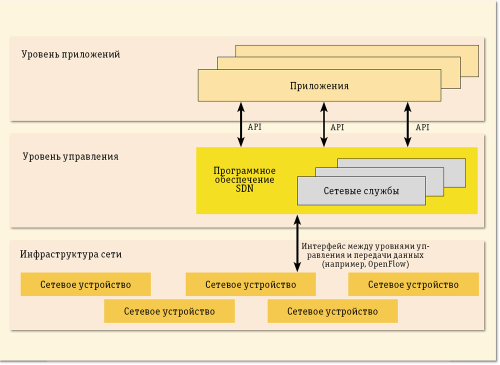
\includegraphics[width=\textwidth]{pic-sdn}
    \caption{Архитектура SDN}\label{fig:pic-sdn}
\end{figure}

\subsection{Протокол OpenFlow}\label{OpenFlow}
Наиболее популярным способом унификации управления программно управляемой сетью вне зависимости от сетевого оборудования является протокол OpenFlow\cite{openflow}, предоставляющий возможности пользователям сети самостоятельно определять и контроллировать трафик и взаимосвязи между участниками компьютерной сети. А также управлять пропускной способностьюи качеством связи между узлами сети. Данный протокол поддерживает три типа сообщений:
\begin{enumerate}
    \item Сообщения, имеющие тип контроллер-коммутатор необходимы для непосредственного управления коммутатором посредством контроллера. Используются для конфигурирования коммутатора, модификации, добавления и удаления записей из таблицы потоков. Инициируется контроллером.
    \item Асинхронные сообщения служат для оповещения контроллера о тех или иных событиях, произошедших в сети. Инициируются коммутатором при прибытии пакета данных или изменения состояния какого-либо узла сети.
    \item Симметричные сообщения инициируются коммутатором или контроллером без необходимости запроса. Используются при установлении соединения, измерения пропускной способности, качества связи и задержек в соединении.
\end{enumerate}

\subsection{Сетевая операционная система (NOS)}\label{nos}
Централизованное управление сетевыми данными предполагает вынесения всего функционала управления сетью  на отдельный узел сети, который принято называть контроллером. Контроллер находится под управлением сетевого администратора и представляет из себя отдельный физический сервер.
Управление контроллером происходит посредством одного или более коммутаторов, обычно работающих на протоколе OpenFlow, и содержищих сетевую операционныю систему, задачей которой является предоставление интерфейса для низкоуровневого управления компьютерной сетью, её сегментами и состояниями её узлов, посредством сетевых сервисов, а также высокоуровневое управление сетью и поток данных посредством приложений\cite{tadviser}.

Сетевая операционная система также способствует обеспечениюю доступа к управлению сетью с помощью приложений и отслеживанию конфигурацию средств сети в режиме реального времени.

Аналогично операционной системе, в традиционном ее понятии, NOS обеспечивает программный интерфейс (API) для управления сетью, а также реализует механизмы управления таблицами коммутаторов: добавление, удаление, изменение правил и сбор статистики. 

Ввиду этого, решение задач управления сетью выполняется фактически с помощью приложений, реализованных на основе программного интерфейса NOS, позволяющего оперировать высокоуровневыми понятиями, такими как имя пользователя или узда, а не низкоуровневыми параметрами конфигурациями, такими как IP-адрес или MAC-адрес.
Это способствует более высокой абстракции над топологией компьютерной сети, однако необходимым условием является то, что сетевая операционная система должна поддерживать отображения между низкоуровневой конфигурацией и её высокоуровневой абстракцией.

\section{Эмуляция компьютерной сети}\label{emulation}
\subsection{Mininet}\label{mininet}
Mininet~-- это эмулятор компьютерной сети, включающей в себя не только хосты и коммутаторы, а также контроллеры. Это программное обеспечение позволяет разворачивать сети из произвольного количества хостов, коммутаторов в различных топологиях в рамках одной виртуальной среды. На всех узлах допускается изменение сетевой конфигурации, а также возможность использования стандартных средств, таких как ipconfig и ping. Помимо этого имеется возможность доступа к терминалу каждого узла сети. Предоставляется возможность управления трафиком через коммутаторы путем задания различных правил маршрутизации и обработки данных.

Ядром Linux, начиная с версии 2.6.24, поддерживаются механизм виртуализации~-- Cgroups\cite{cgroups}, который обеспечивает  процессы сетевыми интерфейсами и таблицами маршрутизации в рамках одной операционной системы. 
Данный механизм виртуализации позвляет запустить несколько процессов в рамказ операционной системы в изолированном окружении, что позволяет Mininet создавать коммутаторы, OpenFlow-контроллеры и хосты, а также взаимодействовать в рамках сети, смоделированной в изолированной среде. Исходый код Mininet написан на Python, за исключением некоторых системных утилит. В рамках этого эмулятора можно описать любую топологию на язке Python. Вся работа с Mininet происходит в рамках командного эмулятора mn~\ref{fig:mn}.
\begin{figure}[H]
    \centering
    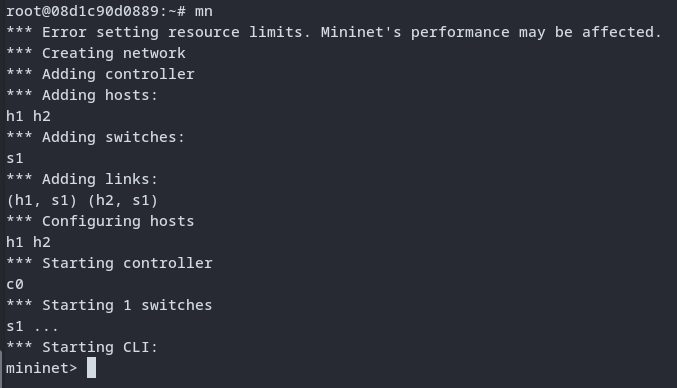
\includegraphics[width=\textwidth]{mn}
    \caption{Командный эмулятор mn}\label{fig:mn}
\end{figure}

По-умолчанию, без дополнительных параметров программное обеспечение переходит в режим интерпретатора команд. Эмулируется компьютерная сеть, состоящая из двух хостов, коммутатора и и контроллера, если в параметрах запускане указано иное.

Mininet предоставляет некоторые собственные команды  для управления виртуальной компьютерной сетью. Ниже приведены некоторые из возможностей\cite{mininet}.

Команда nodes повзялет вывести список узлов всех типов, зарегистрированных в данной сети~\ref{fig:mn-nodes}.
\begin{figure}[H]
    \centering
    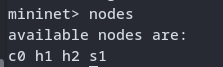
\includegraphics[width=\textwidth]{mn-nodes}
    \caption{Список хостов}\label{fig:mn-nodes}
\end{figure}

Команда net позмоляет посмотреть текущую топологию сети и сопоставление портов коммутатора и хостов~\ref{fig:mn-net}.
\begin{figure}[H]
    \centering
    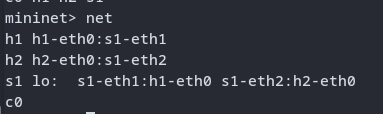
\includegraphics[width=\textwidth]{mn-net}
    \caption{Топология сети}\label{fig:mn-net}
\end{figure}

Команда ifconfig, по аналогии со стоим системным аналогом предоставляет возможность вывода конфигурации сетевого интерфейса конкретного узла сети~\ref{fig:mn-ifconfig}.
\begin{figure}[H]
    \centering
    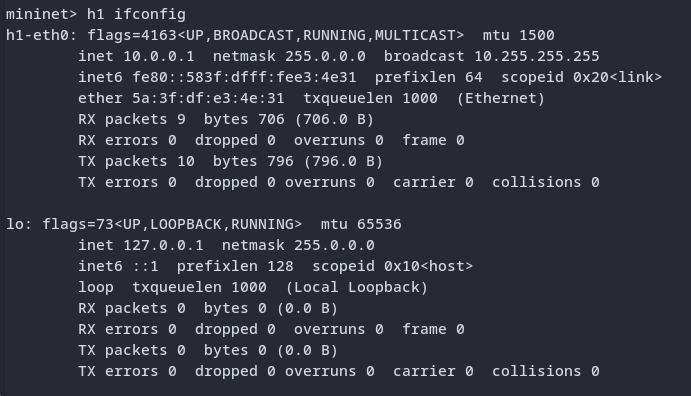
\includegraphics[width=\textwidth]{mn-ifconfig}
    \caption{Конфигурация сетевого интерфейса}\label{fig:mn-ifconfig}
\end{figure}

С помощью команды link можно управлять состоянием любого из портов~\ref{fig:mn-link}.
\begin{figure}[H]
    \centering
    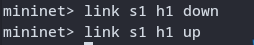
\includegraphics[width=\textwidth]{mn-link}
    \caption{Управление портами коммутатора}\label{fig:mn-link}
\end{figure}

Команда route, аналогично системной команде ядра Linux позволяет просмотреть таблицу маршрутизации для узла  созданной виртуальной компьютерной сети~\ref{fig:mn-route}.
\begin{figure}[H]
    \centering
    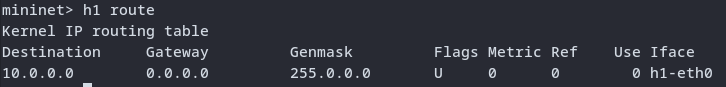
\includegraphics[width=\textwidth]{mn-route}
    \caption{Таблица маршрутизации}\label{fig:mn-route}
\end{figure}

Также предоставляется привычная команда ping~\ref{fig:mn-ping}.
\begin{figure}[H]
    \centering
    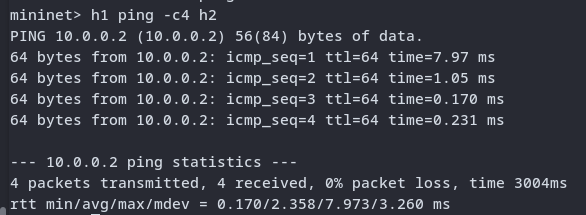
\includegraphics[width=\textwidth]{mn-ping}
    \caption{Пинг}\label{fig:mn-ping}
\end{figure}

А также команда pingall~\ref{fig:mn-pingall}.
\begin{figure}[H]
    \centering
    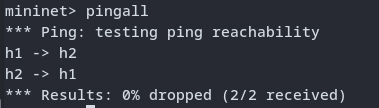
\includegraphics[width=\textwidth]{mn-pingall}
    \caption{Пинг каждого с каждым}\label{fig:mn-pingall}
\end{figure}

Доступна возможность тестирования пропускной способности сети с помощьюкоманды iperf~\ref{fig:mn-ipref}.
\begin{figure}[H]
    \centering
    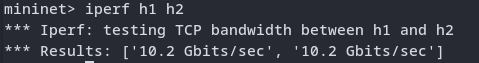
\includegraphics[width=\textwidth]{mn-iperf}
    \caption{Пропускная способность между узлами}\label{fig:mn-iperf}
\end{figure}

Топология сети определяет количество узлов того или иного типа в виртуальной сети. С этого начинается эмуляция компьютерной сети посредством Mininet

Из коробки Mininet предлагает четыре варианта топологии создаваемой сети.
\begin{enumerate}
    \item minimal~-- конфигурация по-умолчанию. Создается два хоста, коммутатор и OpenFlow-контроллер~\ref{fig:mn-minimal}.
    \begin{figure}[H]
        \centering
        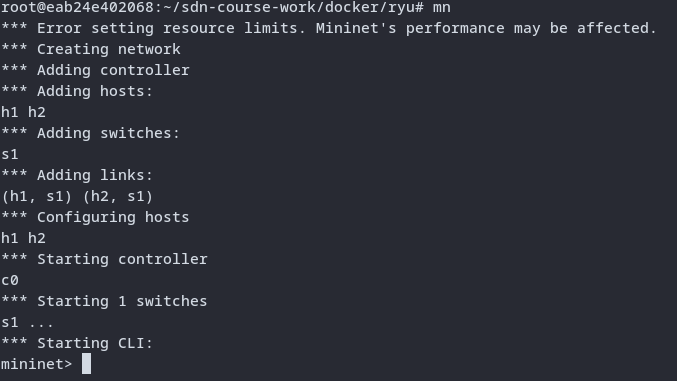
\includegraphics[width=\textwidth]{mn-minimal}
        \caption{Minimal топология}\label{fig:mn-minimal}
    \end{figure}
    \item single~-- аналогично конфигурации minimal, но предоставляется возможность указать количество хостов~\ref{fig:mn-single}.
    \begin{figure}[H]
        \centering
        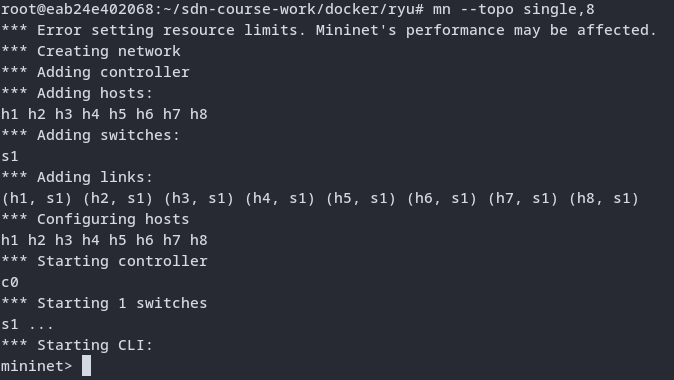
\includegraphics[width=\textwidth]{mn-single}
        \caption{Single топология}\label{fig:mn-single}
    \end{figure}
    \item linear~-- топология, при которой каждый хост подключен к собственному коммутатору, которые в свою очередь соединены между собой~\ref{fig:mn-linear}.
    \begin{figure}[H]
        \centering
        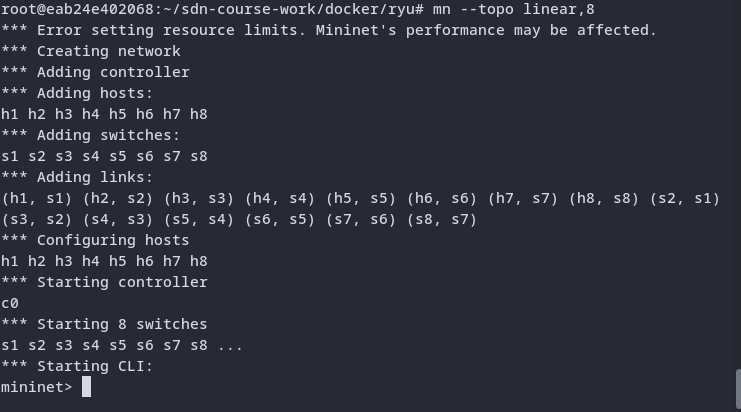
\includegraphics[width=\textwidth]{mn-linear}
        \caption{Линейная топология}\label{fig:mn-linear}
    \end{figure}
    \item tree~-- Древовидная топология, дополнительные параметры указывают глубину иерархии коммутаторов и число подключенных хостов~\ref{fig:mn-tree}.
    \begin{figure}[H]
        \centering
        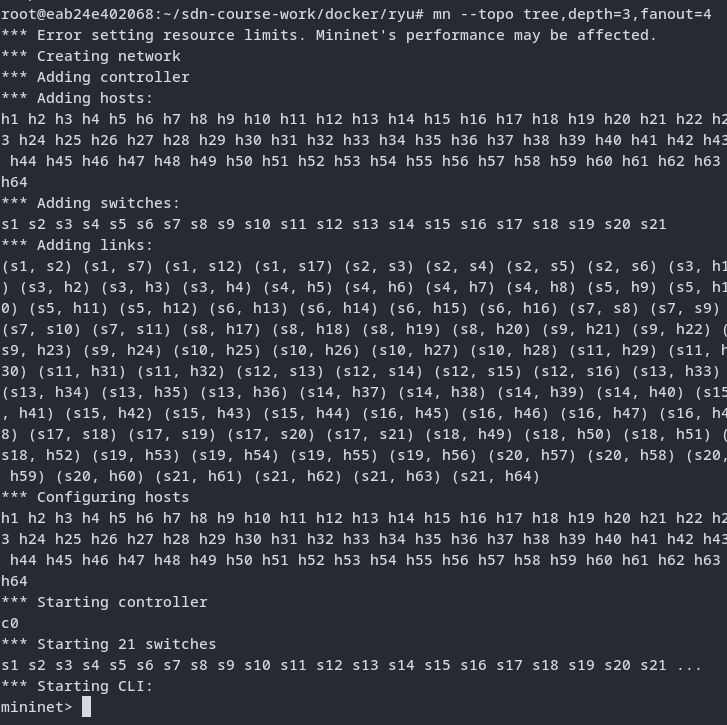
\includegraphics[width=\textwidth]{mn-tree}
        \caption{Древовидная топология}\label{fig:mn-tree}
    \end{figure}
\end{enumerate}

\subsection{Задание топологии сети}\label{topology}
Также доступна возможность создание собственной топологии, описанной на языке Python с помощью ключе --custom
Сделать это можно используя следующую команду запуска~\ref{fig:mn-custom}.
\begin{figure}[H]
    \centering
    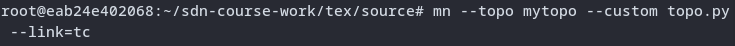
\includegraphics[width=\textwidth]{mn-custom}
    \caption{Собственная топология}\label{fig:mn-custom}
\end{figure}
В файле topo.py описывается структура виртуальной компьютерной сети на языке Python.

\lstinputlisting[firstline=3, lastline=48]{source/topo.py}

После выполнения данного скрипта создается сетьсо следующей топологией~\ref{fig:mn-topo}
\begin{figure}[H]
    \centering
    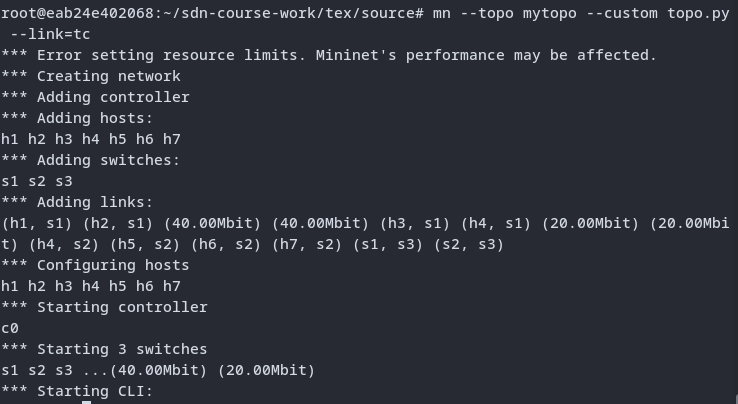
\includegraphics[width=\textwidth]{mn-topo}
    \caption{Топология сети}\label{fig:mn-topo}
\end{figure}

Полный код программы приведен в приложении~\ref{app:topo}.

% -------------------------------
% Раздел "Заключение"
\conclusion
В ходе курсовой работы были описаны недостатки текущей сетевой архитектуры и рассмотрен новый подход к управлению компютерными сетями с помощью программно управляемых сетей и средств виртуализации сетевых функций. Также было рассмотрено программное обеспечение для эмуляции сети с различной топологией и возможностью поледующего управления этой сетью выше описанной технологией SDN.  

% Список литературы
\bibliographystyle{gost780uv}
\bibliography{thesis}

% Окончание основного документа и начало приложений
% Каждая последующая секция документа будет являться приложением

\appendix
\section{Декларативное описание топологии сети}\label{app:topo}
\lstinputlisting[firstline=0, lastline=51]{source/topo.py}

\section{USB-накопитель с отчетом о выполненной работе}\label{app:USB}
На приложенном USB-накопителe можно ознакомиться со следующими файлами:
\begin{description}
\item[Папка \texttt{tex}] "--- \LaTeX- вариант курсовой работы;
\item[\texttt{SoftwareDefinedNetworks.pdf}] "--- курсовая работа.
\item[\texttt{typo.py}] "--- описание топологии сети на языке Python.
\end{description}

\end{document}
